% ICLR full-width motivation figure; generated by scripts/plot_longtail_motivation_v3.py.
\begin{figure*}[t]
  \centering
  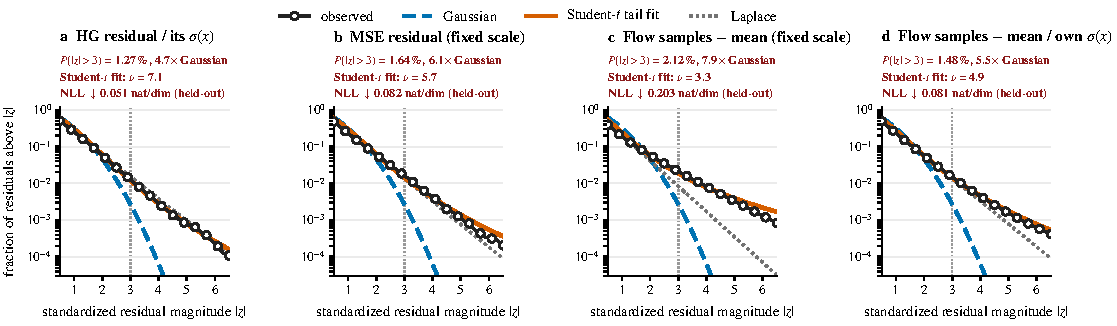
\includegraphics[width=\textwidth]{analysis/paper/longtail_motivation/fig_longtail_motivation_v4.pdf}
  \caption{\textbf{Residuals are heavier-tailed than Gaussian.} Fraction of standardized residual coordinates with magnitude above $|z|$, on
  1{,}728 BridgeData~V2 / WidowX states (eight-step chunks of the six continuous action channels), each model under its
  own scale assumption: \textbf{(a)} a heteroscedastic Gaussian head's residual divided by its predicted $\sigma(x)$;
  \textbf{(b)} an MSE head's residual with one fixed scale; \textbf{(c)} the deviation of each of 1{,}024 Flow samples from
  their per-state mean with one fixed scale; \textbf{(d)} the same deviations divided by the Flow model's own
  conditional scale, the spread of its 1{,}024 samples at that state; coordinate scales are estimated on held-out
  episodes. The gap between (c) and (d) is the state-dependent part of the Flow spread. References: the
  standard normal, a Laplace with the same mean absolute value, and a Student-$t$ matched to the tail. Boxes give the
  share of events beyond $3\sigma$ against the Gaussian 0.27\%, the fitted tail index $\nu$ (7.1, 5.7, 3.3, 4.9), and the
  held-out likelihood gain of a Student-$t$ over a Gaussian. All four decay roughly exponentially, far above the Gaussian: a Gaussian likelihood over-penalizes these events
  while a moderate-$\nu$ Student-$t$ does not.}
  \label{fig:longtail-motivation}
\end{figure*}
